% Options for packages loaded elsewhere
\PassOptionsToPackage{unicode}{hyperref}
\PassOptionsToPackage{hyphens}{url}
%
\documentclass[
]{article}
\usepackage{amsmath,amssymb}
\usepackage{lmodern}
\usepackage{ifxetex,ifluatex}
\ifnum 0\ifxetex 1\fi\ifluatex 1\fi=0 % if pdftex
  \usepackage[T1]{fontenc}
  \usepackage[utf8]{inputenc}
  \usepackage{textcomp} % provide euro and other symbols
\else % if luatex or xetex
  \usepackage{unicode-math}
  \defaultfontfeatures{Scale=MatchLowercase}
  \defaultfontfeatures[\rmfamily]{Ligatures=TeX,Scale=1}
\fi
% Use upquote if available, for straight quotes in verbatim environments
\IfFileExists{upquote.sty}{\usepackage{upquote}}{}
\IfFileExists{microtype.sty}{% use microtype if available
  \usepackage[]{microtype}
  \UseMicrotypeSet[protrusion]{basicmath} % disable protrusion for tt fonts
}{}
\makeatletter
\@ifundefined{KOMAClassName}{% if non-KOMA class
  \IfFileExists{parskip.sty}{%
    \usepackage{parskip}
  }{% else
    \setlength{\parindent}{0pt}
    \setlength{\parskip}{6pt plus 2pt minus 1pt}}
}{% if KOMA class
  \KOMAoptions{parskip=half}}
\makeatother
\usepackage{xcolor}
\IfFileExists{xurl.sty}{\usepackage{xurl}}{} % add URL line breaks if available
\IfFileExists{bookmark.sty}{\usepackage{bookmark}}{\usepackage{hyperref}}
\hypersetup{
  pdftitle={U.S. Education-Energy Poverty Nexus},
  hidelinks,
  pdfcreator={LaTeX via pandoc}}
\urlstyle{same} % disable monospaced font for URLs
\usepackage[margin=1in]{geometry}
\usepackage{graphicx}
\makeatletter
\def\maxwidth{\ifdim\Gin@nat@width>\linewidth\linewidth\else\Gin@nat@width\fi}
\def\maxheight{\ifdim\Gin@nat@height>\textheight\textheight\else\Gin@nat@height\fi}
\makeatother
% Scale images if necessary, so that they will not overflow the page
% margins by default, and it is still possible to overwrite the defaults
% using explicit options in \includegraphics[width, height, ...]{}
\setkeys{Gin}{width=\maxwidth,height=\maxheight,keepaspectratio}
% Set default figure placement to htbp
\makeatletter
\def\fps@figure{htbp}
\makeatother
\setlength{\emergencystretch}{3em} % prevent overfull lines
\providecommand{\tightlist}{%
  \setlength{\itemsep}{0pt}\setlength{\parskip}{0pt}}
\setcounter{secnumdepth}{-\maxdimen} % remove section numbering
\usepackage{booktabs}
\usepackage{longtable}
\usepackage{array}
\usepackage{multirow}
\usepackage{wrapfig}
\usepackage{float}
\usepackage{colortbl}
\usepackage{pdflscape}
\usepackage{tabu}
\usepackage{threeparttable}
\usepackage{threeparttablex}
\usepackage[normalem]{ulem}
\usepackage{makecell}
\usepackage{xcolor}
\ifluatex
  \usepackage{selnolig}  % disable illegal ligatures
\fi

\title{U.S. Education-Energy Poverty Nexus}
\author{true}
\date{2021-11-29}

\begin{document}
\maketitle

\hypertarget{introduction}{%
\subsection{Introduction}\label{introduction}}

\textbf{Premise:} Energy poverty is one of the significant challenges
for developing countries of the world with more than a billion people
around the world lacking access to simple technologies such as lamps and
appliances. The idea that the lack of access to lighting at night or
heating/cooling during thermal comfort could impact children and their
ability to perform well in school seems apparent. Several studies have
concluded households with a low level of educational attainment have
more limited access to electricity and other forms of clean energy
(Apergis, Polemis, and Soursou 2021). It's evident that there's
potential for a vicious cycle where energy poverty is hindering
education which in turn decreasing their ability to escape it; ultimate
depriving people of a higher quality life.

\textbf{Question:} Do these relationships between energy poverty and
education hold true in the United States (the developed country context,
based on GDP)?

\textbf{Motivation:} There is a lack of research connecting education
and energy poverty in the US. Though electricity access is prevalent in
the U.S., anticipated increased variability in climate could make the
U.S. particularly vulnerable. The disparities in energy equity
considering income and race across the US are not recognized as a
problem at the federal level, therefore limiting the response to this
issue unlike the gradual and coordinated response in countries such as
the UK (Bednar and Reames 2020). The goal of this project is to
encourage more research through the education-energy poverty nexus lens.

\hypertarget{datasets-used}{%
\subsection{Datasets Used}\label{datasets-used}}

The analysis was conducted on the county level in the US due to the
increased sampling power and available data resolution for parameters in
question.

\textbf{Educational Attainment data} available on the county-level from
the USDA Economic Research Service, the most recent data is available
for 2015 to 2019 (Link:
\url{https://data.ers.usda.gov/reports.aspx?ID=17829} )
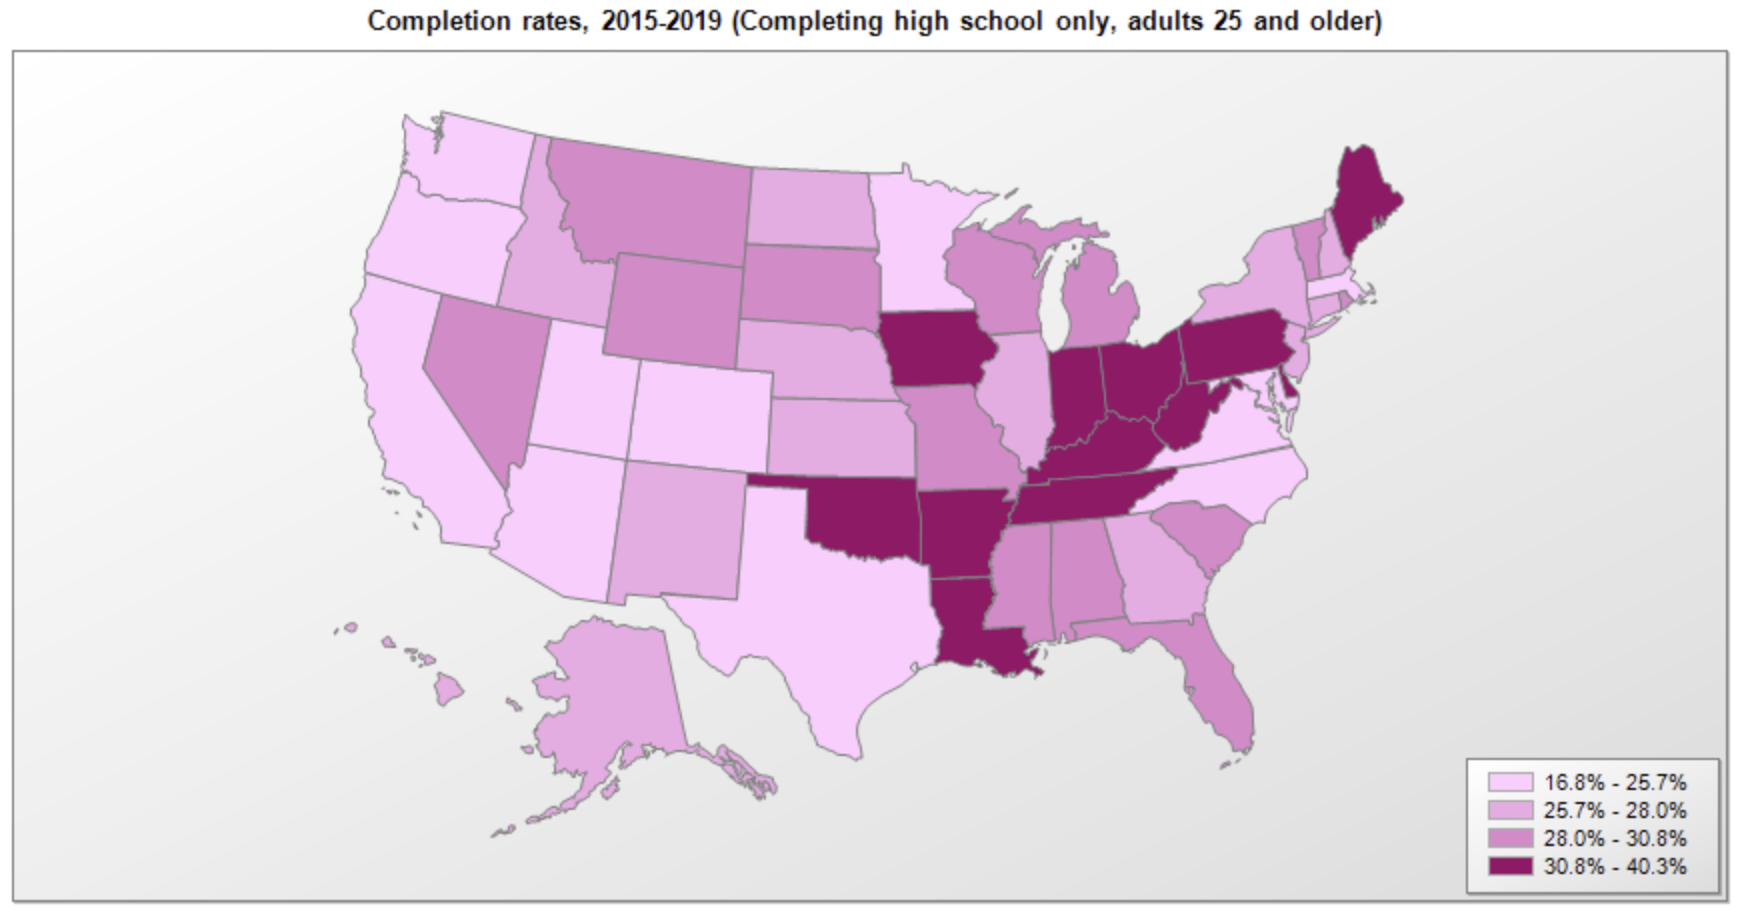
\includegraphics{img/educ-attainment.png} \textbf{Comprehensive County
Indicators data} from County Health Rankings which compiles data from
several data sources. The final analysis used the \textbf{\emph{math and
reading score indicators}} from this dataset that are modelled by
Stanford Education Data Archive program based on EDFacts and state
sources to achieve comparability across the country. Although the
dataset is labelled as 2021 data, the testing score is actually based on
2018. The math and reading scores are presented as average grade level
performance for 3rd graders. The scores generally range from 1 to 4. The
expected value is 3 indicating that 3rd graders are performing at a 3rd
grade level. A score of 3.5 would they are perform 0.5 a grade level
higher than expected. (Link:
\url{https://www.countyhealthrankings.org/explore-health-rankings/rankings-data-documentation})

\textbf{Low-Income Energy Affordability data} available on county-level
from the Department of Energy based on modelling done using the 2016
5-year American Community Survey (ACS5) (Link:
\url{https://www.energy.gov/eere/slsc/low-income-energy-affordability-data-lead-tool})
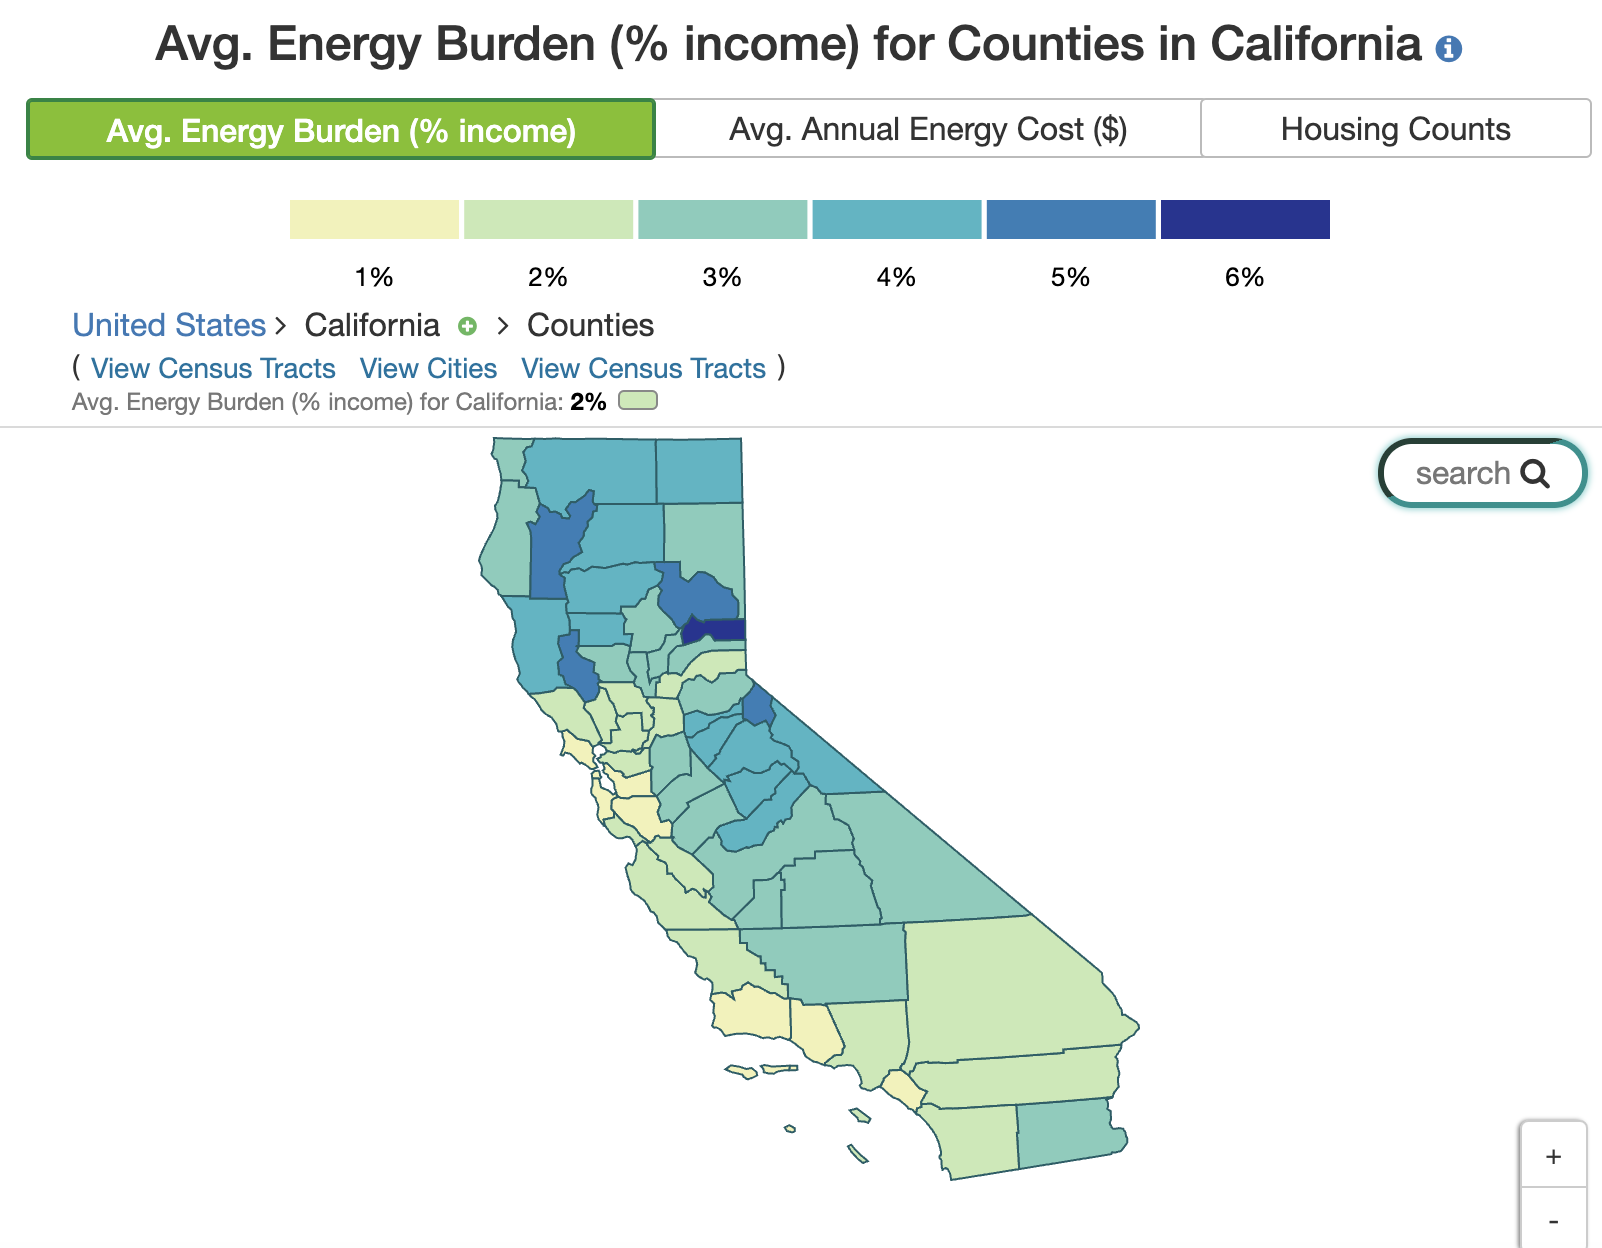
\includegraphics{img/CA-lead-tool-map.png} \textbf{Limitations of the
the datasets used}:

The LEAD energy affordability estimates are centered around housing
energy costs. While this is important, an entire dimension of inequity
due to energy poverty and mobility is missed out on due to the lack of
information on transportation sector.

With county-level resolution in US being so challenging to achieve, it's
important to note that there are several processes of modelling and
estimations incorporated into the available datasets for the education
data and LEAD tool that must be considered and noted. Biases could arise
due to response bias and attrition for the surveys such as the American
Community Survey (ACS) that are heavily relied on.

Nevertheless, this analysis will use the best available data to my
knowledge for reasonably overlapping time periods.

\hypertarget{analysis-plan}{%
\subsection{Analysis Plan}\label{analysis-plan}}

There will be two stages to the analysis.

\hypertarget{part-1}{%
\subsubsection{Part 1}\label{part-1}}

First will be exploring whether there is a correlation between
educational attainment and energy burden.

\textbf{How does educational attainment affect energy burden?}

The Apergis, Polemis, and Soursou 2021 paper concluded that across
several energy poverty and education studies in developing countries
that ``households with a low level of educational attainment, have
restricted access to clean energy forms, such as electricity''. In the
developed country context, we will test if a similar relationship exists
between educational attainment and energy burden. The assumption is that
\textbf{energy burden} is a representative measure of access instead of
the binary ``access/no access'' scenario in developing countries.

\[\text{energy burden}_i = \beta_0 + \beta_1 \text{educational attainment}_i + \epsilon_i\]
\textbf{Energy burden will be represent by the average energy burden (\%
Income)} from the LEAD Energy Affordability data \textbf{Educational
attainment will be represented by the \% of adults with a HS diploma or
less} from USDA Economic Research Service data

\hypertarget{part-2}{%
\subsubsection{Part 2}\label{part-2}}

Next we will be exploring whether there is a correlation between energy
burden and educational outcomes(measured by standardized math and
reading scores). The idea is that examining a short-term education
measure such as standardized test scores will reflect the effects of
energy burden as surveyed and modeled in recent data.

\textbf{Does energy burden affect a student's ability to do well in
school?}

The assumption is that 3rd grader \textbf{english and math standardized
test scores} are a representative measure of doing well in school.

With the energy affordability data mainly reflecting household building
energy needs, it is expected that heating and cooling dominates energy
spending. US Energy Information Administration estimates that more that
half of household energy spending is spent on heating and cooling. The
lack of thermal comfort has shown to increase the amount of mistakes by
even adults. The Institute of Education Sciences has compiled literature
on the optimal learning temperature based on thermal comfort
(\url{https://ies.ed.gov/ncee/edlabs/regions/west/Ask/Details/64}).

The rationale is that although most families in America have access to
electricity and basic technologies such as lighting and temperature
regulation, they may be unable to take full advantage of them due to the
energy burden.

\[\text{standardized test scores-READING}_i = \beta_0 + \beta_1 \text{energy burden}_i + \epsilon_i\]
\[\text{standardized test scores-MATH}_i = \beta_0 + \beta_1 \text{energy burden}_i + \epsilon_i\]
\textbf{Standardized test scores will be represented by the math and
reading scores presented as average grade level performance for 3rd
graders} from Stanford Education Data Archive data accessed through
County Health Rankings \textbf{Energy burden will be represent by the
average energy burden (\% Income)} from the LEAD Energy Affordability
data

\hypertarget{results}{%
\subsection{Results}\label{results}}

\begin{table}

\caption{\label{tab:unnamed-chunk-3}**Does educational attainment affect energy burden?**}
\centering
\begin{tabular}[t]{l|r|r|r|r}
\hline
  & Estimate & Std. Error & t value & Pr(>|t|)\\
\hline
(Intercept) & 1.111 & 0.096 & 11.553 & 0\\
\hline
pct\_hs\_or\_less & 0.062 & 0.002 & 31.206 & 0\\
\hline
\end{tabular}
\end{table}

\textbf{Answer: Since \(p-value is < 0.001\) we reject the null that
educational attainment(\% with HS diploma or less) has an effect of 0 on
Average Energy Burden(\% Income).} We can say there is a
\textbf{statistically significant correlation (at the 0.1\% significance
level).}

The \(\beta_1\) indicates that there is \textbf{0.062 increase in
average energy burden as \% Income for every percent point increase in
\% with HS diploma or less} in a given a county.

Although the estimated coefficient is positive, it is truly reflecting a
negative correlation between educational attainment and energy burden.
Since the educational attainment variable used is \% with a high school
diploma or less, an increase in this variable indicates less education
attained. Therefore, with less education attained, there is an increase
in energy burden.

\begin{table}

\caption{\label{tab:unnamed-chunk-4}**Does energy burden affect reading scores (among 3rd graders)?**}
\centering
\begin{tabular}[t]{l|r|r|r|r}
\hline
  & Estimate & Std. Error & t value & Pr(>|t|)\\
\hline
(Intercept) & 3.243 & 0.016 & 200.764 & 0\\
\hline
avg\_energy\_burden\_percent\_income & -0.059 & 0.004 & -15.377 & 0\\
\hline
\end{tabular}
\end{table}
\begin{table}

\caption{\label{tab:unnamed-chunk-5}**Does energy burden affect math scores (among 3rd graders)?**}
\centering
\begin{tabular}[t]{l|r|r|r|r}
\hline
  & Estimate & Std. Error & t value & Pr(>|t|)\\
\hline
(Intercept) & 3.233 & 0.019 & 170.446 & 0\\
\hline
avg\_energy\_burden\_percent\_income & -0.063 & 0.005 & -14.016 & 0\\
\hline
\end{tabular}
\end{table}

\textbf{Answer: Since \(p-value is < 0.001\) we reject the null that
there is that Average Energy Burden(\% Income) has an effect of 0 on
standardized test scores.} We can say there is a \textbf{statistically
significant correlation (at the 0.1\% significance level).}

The \(\beta_1\) indicates that there is \textbf{0.06 decrease in average
grade level in reading and math scores for every percent point increase
in average energy burden as \% Income} in a given a county.

\hypertarget{conclusions-and-next-steps}{%
\subsection{Conclusions and Next
steps}\label{conclusions-and-next-steps}}

The two-step analysis indicated that lower levels educational attainment
correlate with higher levels of energy burden and higher levels of
energy burden correlate with lower standardized test scores. This
indicates there may be a cycle of energy poverty that is difficult to
break through because of it's close linkage with education. To confirm
this connection, further research is needed to scrutinize the existing
models. With the lows R\^{}2 values, the current models are far from
being predictive. Further evidence is needed to determine whether energy
burdens are affecting school performance through thermal comforts or
some other means.

Starting points could be:

\begin{enumerate}
\def\labelenumi{\arabic{enumi}.}
\item
  Are there any potential omitted variable biases?
\item
  Is energy poverty able to be detached from the effects of poverty and
  income levels as a whole?
\item
  What variables could enable the existing models to be developed into
  predictive models?
\end{enumerate}

Answering these questions could help gather the needed attention on
energy poverty in the US and how a targeted approach could be used to
address the inequities.

\hypertarget{references}{%
\subsection{References}\label{references}}

Apergis, Nicholas, Michael Polemis, and Simeoni-Eleni Soursou. 2021.
``Energy Poverty and Education: Fresh Evidence from a Panel of
Developing Countries.'' Energy Economics, July, 105430.
\url{https://doi.org/10.1016/j.eneco.2021.105430}. Bednar, Dominic J.,
and Tony G. Reames. 2020. ``Recognition of and Response to Energy
Poverty in the United States.'' Nature Energy 5 (6): 432--39.
\url{https://doi.org/10.1038/s41560-020-0582-0}. ``County Health
Rankings 2021: Codebook for Analytic Datasets.'' 2018, 5. ``Does
Temperature Impact Student Performance? \textbar{} Association for
Learning Environments.'' n.d. Accessed November 29, 2021a.
\url{https://healthyschools.cefpi.org/temperature.html}. ``---------.''
n.d. Accessed November 29, 2021b.
\url{https://healthyschools.cefpi.org/temperature.html}. ``Math
Scores\emph{.'' n.d. County Health Rankings \& Roadmaps. Accessed
November 29, 2021.
\url{https://www.countyhealthrankings.org/explore-health-rankings/measures-data-sources/county-health-rankings-model/health-factors/social-and-economic-factors/education/math-scores}.
``Reading Scores}.'' n.d. County Health Rankings \& Roadmaps. Accessed
November 29, 2021.
\url{https://www.countyhealthrankings.org/explore-health-rankings/measures-data-sources/county-health-rankings-model/health-factors/social-and-economic-factors/education/reading-scores}.
University, © Stanford, Stanford, and California 94305. n.d. ``Stanford
Education Data Archive (SEDA).'' Accessed November 29, 2021.
\url{https://purl.stanford.edu/db586ns4974}. ``Use of Energy in Homes -
U.S. Energy Information Administration (EIA).'' n.d. Accessed November
29, 2021.
\url{https://www.eia.gov/energyexplained/use-of-energy/homes.php}.

\end{document}
